\documentclass[a4paper,12pt]{article}
\usepackage{graphicx}
\usepackage[left=30mm, right=30mm, top=30mm, bottom=35mm]{geometry}
\usepackage{amsmath}
\usepackage{siunitx}
\usepackage{fancyhdr}
\usepackage{url}
\pagestyle{fancy}
%-------------------------------------------------------------------------------
\lhead{\textbf{Fall 2019}}
\rhead{\textbf{CE311K Intro to Computer Methods}}
\cfoot{\thepage}
%-------------------------------------------------------------------------------

\begin{document}
\begin{centering}
	\textbf{
		Assignment 06: Solving system of linear equations\\
		Assigned: 3rd December 2019\\
		Due: 9th December 2019 at 5 PM\\
	}
\end{centering}


Note: Please upload your solution as an ipynb file to the Canvas page.

\vspace{1em}
 
 The purpose of this assignment is to introduce you to computer methods for solving systems of

 simultaneous linear equations. You will perform hand calculations that solves the equations using
Gauss Elimination and Gauss-Seidel iterative approach and then and write a computer program that does the same.
 
\begin{enumerate}
	\item Given the system of equations $Ax = b$, as defined below:

	\begin{align*}
	\begin{bmatrix}
	8 & 2 & 3 \\
	2 & 5 & 1 \\
	-3 & 1 & 6 \\
	\end{bmatrix}
	\quad
	\begin{bmatrix}
	x_1 \\
	x_2 \\
	x_3 \\
	\end{bmatrix}
	\quad
	\begin{bmatrix}
	51 \\
	23 \\
	20 \\
	\end{bmatrix}
	\end{align*}
	\begin{enumerate}
		\item Determine the solution by hand using Gauss Elimination
		\item Write a Python code for Gauss Elimination to solve the above equation
		\item Use the `\verb|numpy.linalg.solve|' library function to solve
		\item Carry out three iterations of the Gauss-Seidel method, assuming an initial values of $x$ equal to zero. After the third iteration, compute the error for each estimate with relative to the true values from `\verb|numpy.linalg.solve|'
	\end{enumerate}

	\item Solve the  axial forces $F_i$ for the following truss with pin-joints and 13 members. The resulting system of 13 equations is:
	\begin{figure}[ht]
		\centering
		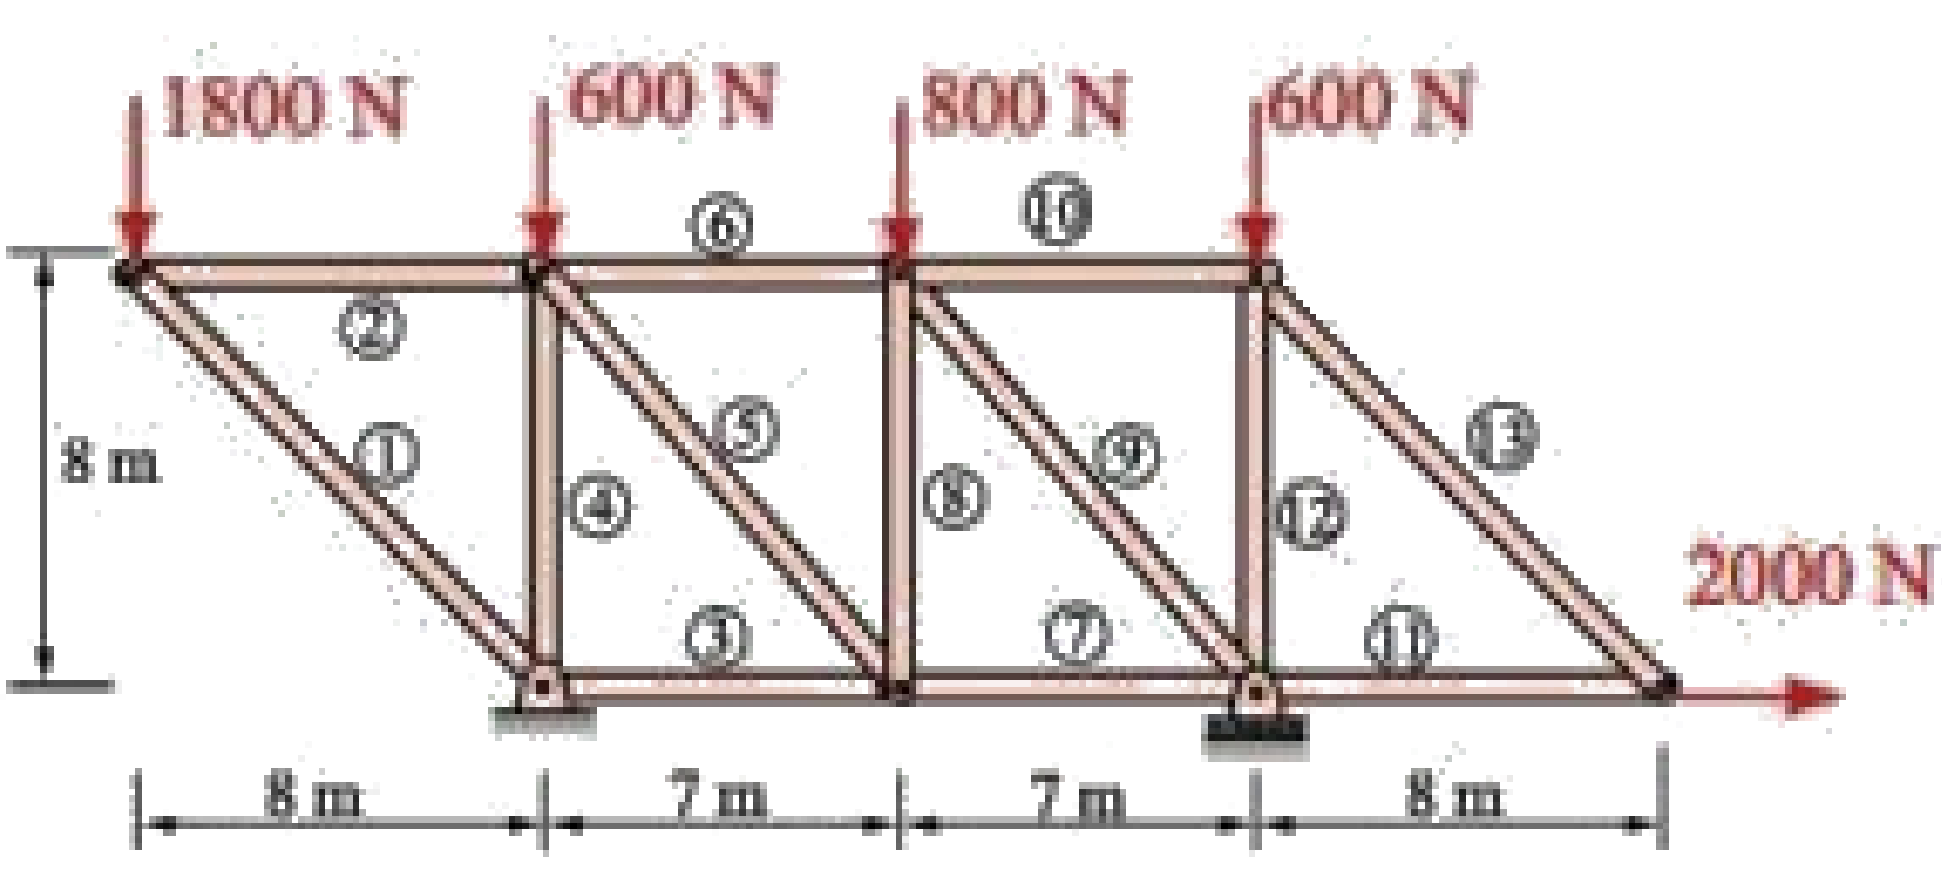
\includegraphics[width=0.7\textwidth]{truss.png}
	\end{figure}
	\begin{align*}
	F_2 + 0.707 F_1 & = 0    \\
	F_3 - 0.707 F_1 - 2000 & = 0\\
	0.707F_1 + F_4 + 6229 & = 0 \\
	-F_2 + 0.659F_5 + F_6 & = 0 \\
	-F_4 - 0.753 F_5 - 600 &  = 0 \\
	-F_3 -0.659F_5 + F_7 & = 0 \\
	F_8 + 0.753F_5 & = 0 \\
	-F_6 + 0.659 F_9 + F_{10} & = 0 \\
	-F_8 -0.753 F_9 - 800 &= 0 \\
	-F_7 -0.659F_9 + F_{11} &= 0 \\
	F_{12} + 0.753 F_9 - 2429 &= 0 \\
	-F_{10} + 0.707 F_{13} & = 0 \\
	-F_{12} - 0.7071 F_{13} - 600 &= 0\\
	\end{align*}
	
	\begin{enumerate}
		\item Solve this system of equations using the solve function in the linalg package from
numpy.
		\item Solve this system of equations using your Gauss-Seidel user defined function using
initial values of $F$ equal to zero. Explain what is happening when you try to solve this
problem using Gauss-Seidel.

	\end{enumerate}
\end{enumerate}

\end{document}

